 
\section{Preliminary Results}
\label{sec:results}

\begin{itemize}
\item need a coherent story here (organize as a story!)
\item show some optimization examples, provide story
\item character of solution(s), observations
\item define how we measure flux!
\end{itemize}

The computer simulations of this proposal are intended to discover the
optimal system configuration for a range of scenarios and system
sizes. The results of these simulations will be used as input for the
design of a pilot site in Mesa, Arizona, and eventually, over a range of
scenarios and system sizes. 

  \begin{figure}[!htb]
   \begin{center}
    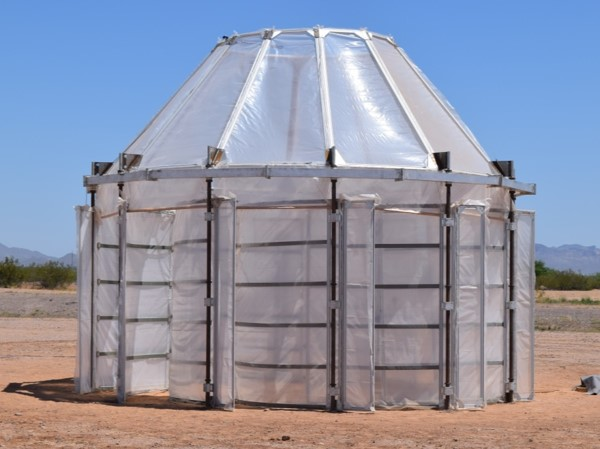
\includegraphics[width = 12 cm]{figs/sov_field}
    \caption{A photo of the field configuration, during the June 2015
    Field Test.}
    \label{fig:field_real}
   \end{center}
  \end{figure}

In addition to the system configuration, it is important to consider the
effect of local conditions on SoV performance. Characterizing the impact
of variations in ambient conditions on the SoV will guide the
commercialization strategy of the product, by determining optimal
install locations across the country. It is therefore desirable to have
models 
that are capable of accounting for variation in field conditions, such
as solar input, cross-winds and topography. Furthermore, it is expected
that large ``farms'' of SoVs (akin to the wind and solar farms for wind
turbines and photovoltaics, respectively) may be used by commercial or
utility-scale energy generation. In order for this to be effective, 
the inter-unit spacing must also be optimized, as a single SoV collects
from a large area. These computations will guide commercialization
planning, where decision-makers will need to assess optimum unit size,
spacing, and geographic location for utility-scale deployment.  

While ambient winds in the field do impact system performance, our
present work focuses on an idealized scenario with natural convection
driven only by thermal instabilities. Investigating this baseline,
thermal-only flow is intended to optimize the SoV apparatus to form a
strong  thermal plume even in the absence of wind. After a system is
engineered to form a strong thermal plume, we will then work to ensure
that the existing thermal vortex will be strengthened by the addition of
winds.     

Results from previous simulations of the straight, multiple tiered vane
systems implied that the inlet angles of the vanes were too severe
versus the ambient flow being drawn into the  apparatus. As a result,
the vanes were blocking the incoming flow, and were resulting in an
adverse pressure gradient existing near the outside edge of the
vanes. This served to force fluid  around and over the system, instead
of inside the turning vanes. This reduces the velocity of flow  inside
the system, resulting in a weaker thermal vortex.  In order to reduce
the flow blockage, we have begun to experiment with curved vanes. The
intent behind this change from the straight vanes is to reduce the inlet
angle. A gentler angle  permits more flow to enter the vane region,
after which the curvature increases toward the center of the vanes. In
this way, the angle smoothly varies between 0 degrees at the outside
edge of the vanes to a maximum angle at a specified inner radius which
depends on the tier of vanes.  Examples of the curved vanes for the top
and bottom levels from the two-tier curved vanes are shown below.  

The bottom tier vanes are designed to be approximately the height of the
boundary layer, and to have a greater final angle than the higher
tier. The inner angle is consistent with the final angle in the bottom
tier for the straight vanes. Likewise, the top tier is designed to have
a similar final angle as the straight vane case.

While these results are promising, the thermal plume is relatively
narrow compared to the diameter of the device. It is desirable to
broaden the thermal plume, as this in turn creates a larger vertical
momentum flux due to the effects of buoyancy. This will presumably
entrain more  surrounding fluid, driving it through the vanes and
imparting kinetic energy to the flow. The kinetic energy grows as the
square of the radius, so any broadening of the vortex core can greatly
enhance the kinetic energy flux.  

As a result, a parallel effort designed to engineer a broader thermal
plume has begun this quarter. The general physical mechanisms that
determine the thermal plume's thickness are not  presently understood,
and so the simulation groups efforts have focused on probing possible
hypotheses through the addition of general forcing of the velocity
field. The driving simulation  software has been modified in order to
permit generic forcing functions that are dependent on spatial location
as well as state variables, such as the velocity field. In this way, an
appropriately  scaling can be applied to the forcing. 

As shown below, this forcing has substantially broadened the thermal
plume as well as lifted the thermal resource from the ground into the
flow. In turn, this has increased the diameter of the dust devil's
core. 

Potential Temperature is defined as,
\begin{equation}
  \theta(x,y,z) = T(x,y,z) -T_{in}(z) 
\end{equation}



%
%\subsection{Character of the Solution}
%
%Talk about how the vortex transitions from phase 1 to 2, etc. 
